\documentclass[tikz]{standalone}
\usepackage{pgfplots}
%\pgfplotsset{compat=1.8}
\begin{document}

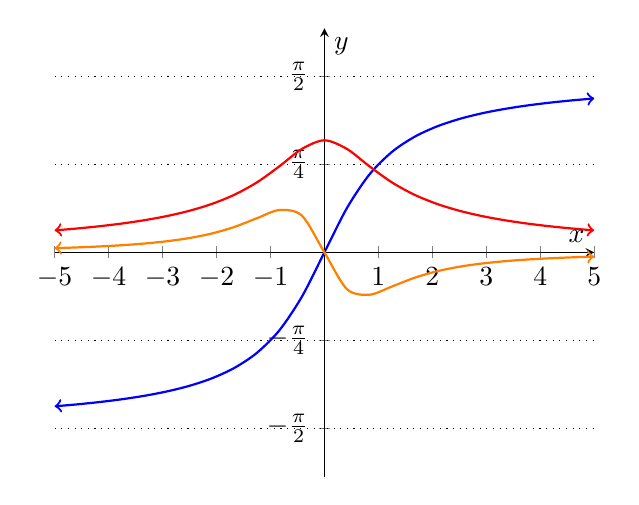
\begin{tikzpicture}[
  declare function={
    % define the arctan function, be sure to include rad() so as radians are used
    arctan(\x)= rad(atan(x));
    % first derivative of arctan(x)
    first(\x)= 1/sqrt(x^2+1);
    % second derivative of arctan(x)
    second(\x) = (-(1/2)*(x^2+1)^(-1/2)*(2*x)) / (x^2+1);
  }
]
\begin{axis}[
  axis x line=middle,
  axis y line=middle,
  xmin=-5, xmax=5, xtick={-5,...,5},
  xlabel=$x$,
  ymin=-2, ymax=2,
  ytick={-1.570796,-0.785398, 0.785398, 1.570796},
  yticklabels={$-\frac{\pi}{2}$,$-\frac{\pi}{4}$,$\frac{\pi}{4}$,$\frac{\pi}{2}$},
  ylabel=$y$,
]

\pgfplotsinvokeforeach{-1.570796, -0.785398, 0.785398, 1.570796 }{
  \draw[dotted] ({axis cs: -5, #1}) -- ({axis cs: 5, #1});}
  
\addplot[<->,blue, domain=-5:5, smooth, thick]{arctan(x)};
\addplot[<->,red, domain=-5:5, smooth, thick]{first(x)};
\addplot[<->,orange, domain=-5:5, smooth, thick]{second(x)};
\end{axis}

\end{tikzpicture}

\end{document}
%sagemathcloud={"zoom_width":80}